\documentclass{beamer}

% Use a modern academic theme (e.g., metropolis)
\usetheme{metropolis}
\usecolortheme{default}
\usepackage{graphicx}
\usepackage{booktabs}
\usepackage{amsmath}
\usepackage{hyperref}
\usepackage{bm}
\usepackage{multirow}

% For highlighting
\newcommand{\alertterm}[1]{\alert{\textbf{#1}}}

% fix: \bench undefined; define it as 'Paper2Video'
\newcommand{\bench}{Paper2Video}

% fix: \Letter undefined for presenter mark
\usepackage{textcomp}
\newcommand{\Letter}{\textsuperscript{\texttildelow}}

% Title and author information
\title[Paper2Video]{
\includegraphics[height=0.6cm]{figure/logo_.png} Paper2Video: Automatic Video Generation from Scientific Papers}
\author[Zeyu Zhu, Kevin Q. Lin, Mike Z. Shou]{
  Zeyu Zhu\textsuperscript{*}, Kevin Qinghong Lin\textsuperscript{*}, Mike Zheng Shou\Letter \\
  {\small Show Lab, National University of Singapore}
}
\date{\today}


\setbeamerfont{caption}{size=\scriptsize}
\begin{document}
\begin{frame}
  \titlepage
\end{frame}

\begin{frame}{Motivation}
  \begin{figure}
      \centering
      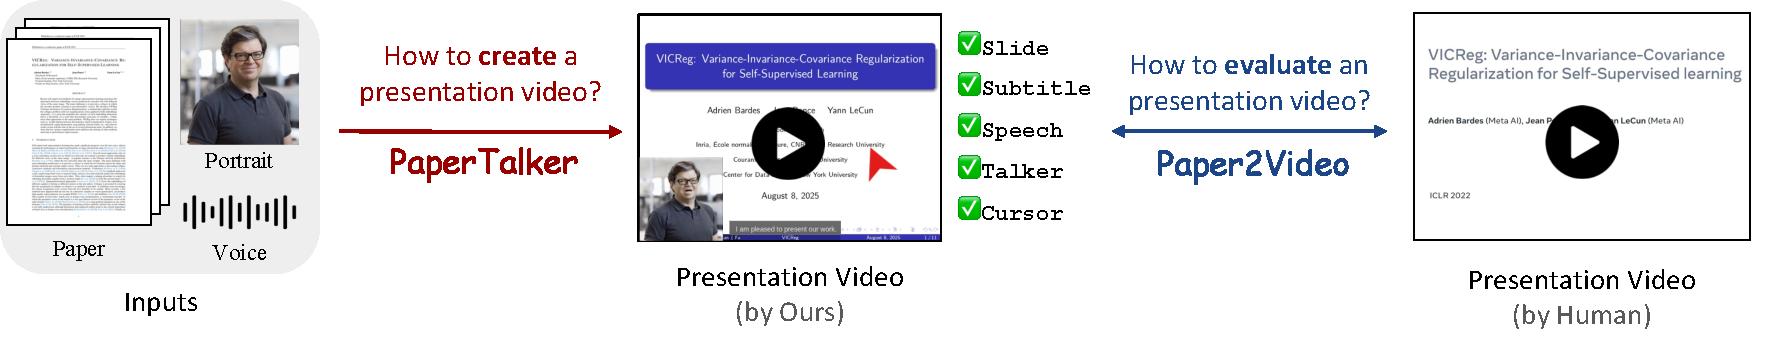
\includegraphics[width=1\linewidth]{figure/teaser.pdf}
      \vspace{-1\baselineskip}
      \label{fig:placeholder}
  \end{figure}
  \vspace{-1\baselineskip}
 \begin{block}{\small Motivation}
 \footnotesize
  \begin{itemize}
    \item \textbf{Academic presentation videos} are widely used for research dissemination, but \alertterm{producing them is highly labor-intensive}.
    \item Manual process involves slide design, recording, subtitling, and editing -- often hours for only a few minutes of video.
    \item \alertterm{Challenge:} Presentation video generation is a complex, multi-modal, long-context task with no existing benchmarks or tailored metrics.
  \end{itemize}
  \end{block}
  \begin{block}{\small Key Questions}
    \footnotesize
    \begin{itemize}
      \item What defines a \alertterm{good academic presentation video}?
      \item How to \alertterm{automatically generate} such a video from a research paper?
    \end{itemize}
  \end{block}
\end{frame}
\begin{frame}{Paper2Video Benchmark}
  \begin{figure}
    \centering
    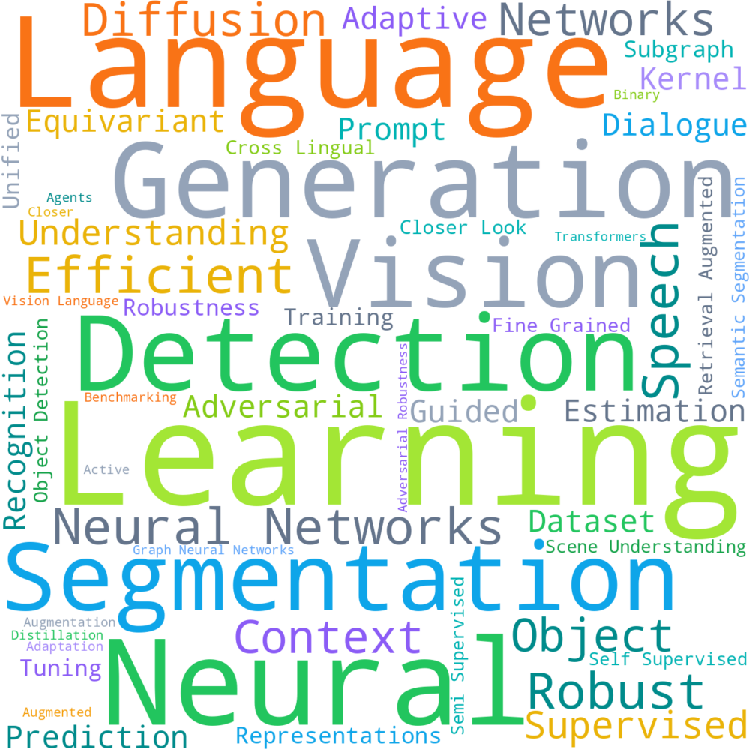
\includegraphics[width=0.30\textwidth]{figure/paper_topics_wordcloud.pdf}
    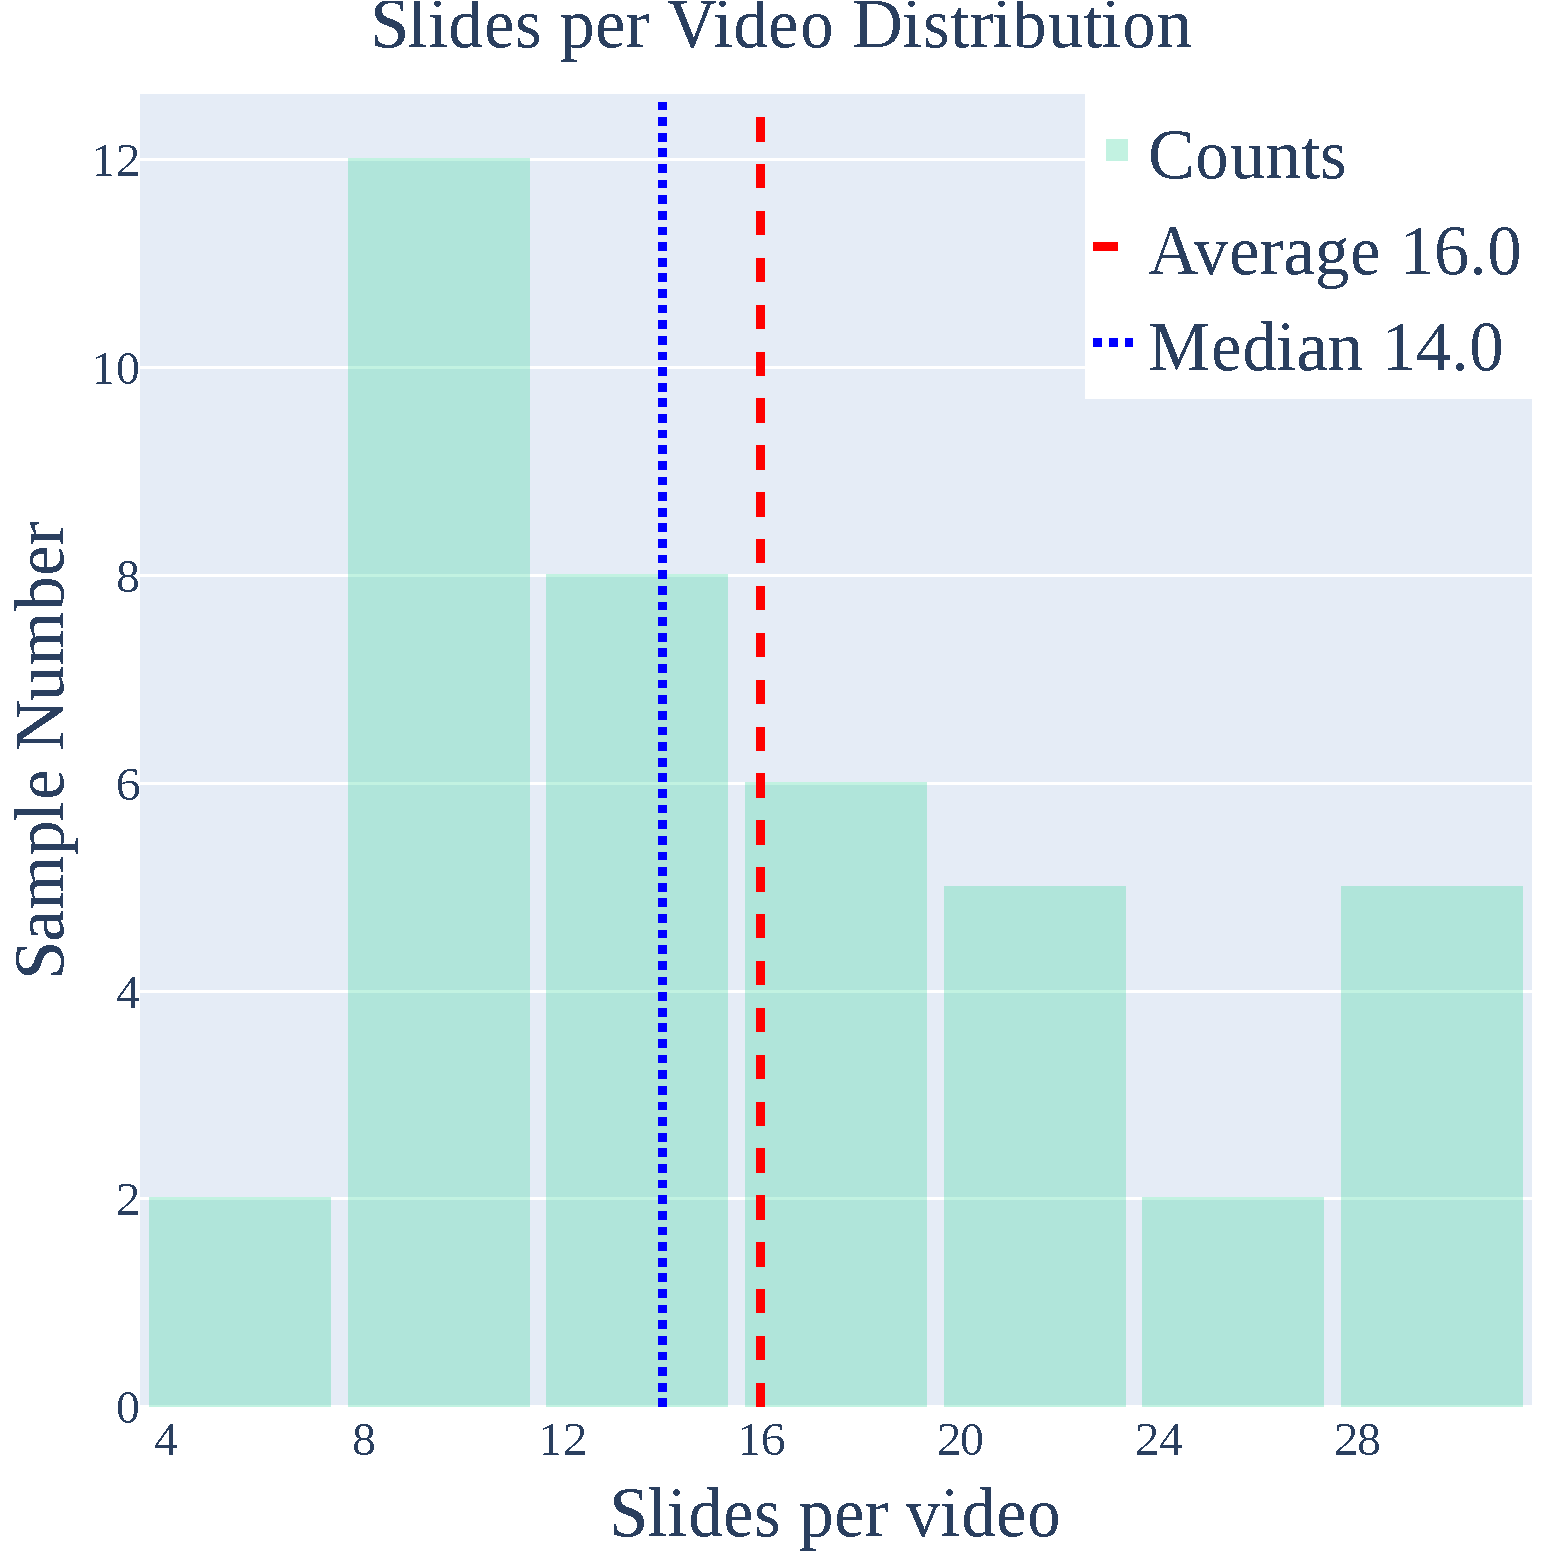
\includegraphics[width=0.30\textwidth]{figure/slides_count_hist.pdf}
    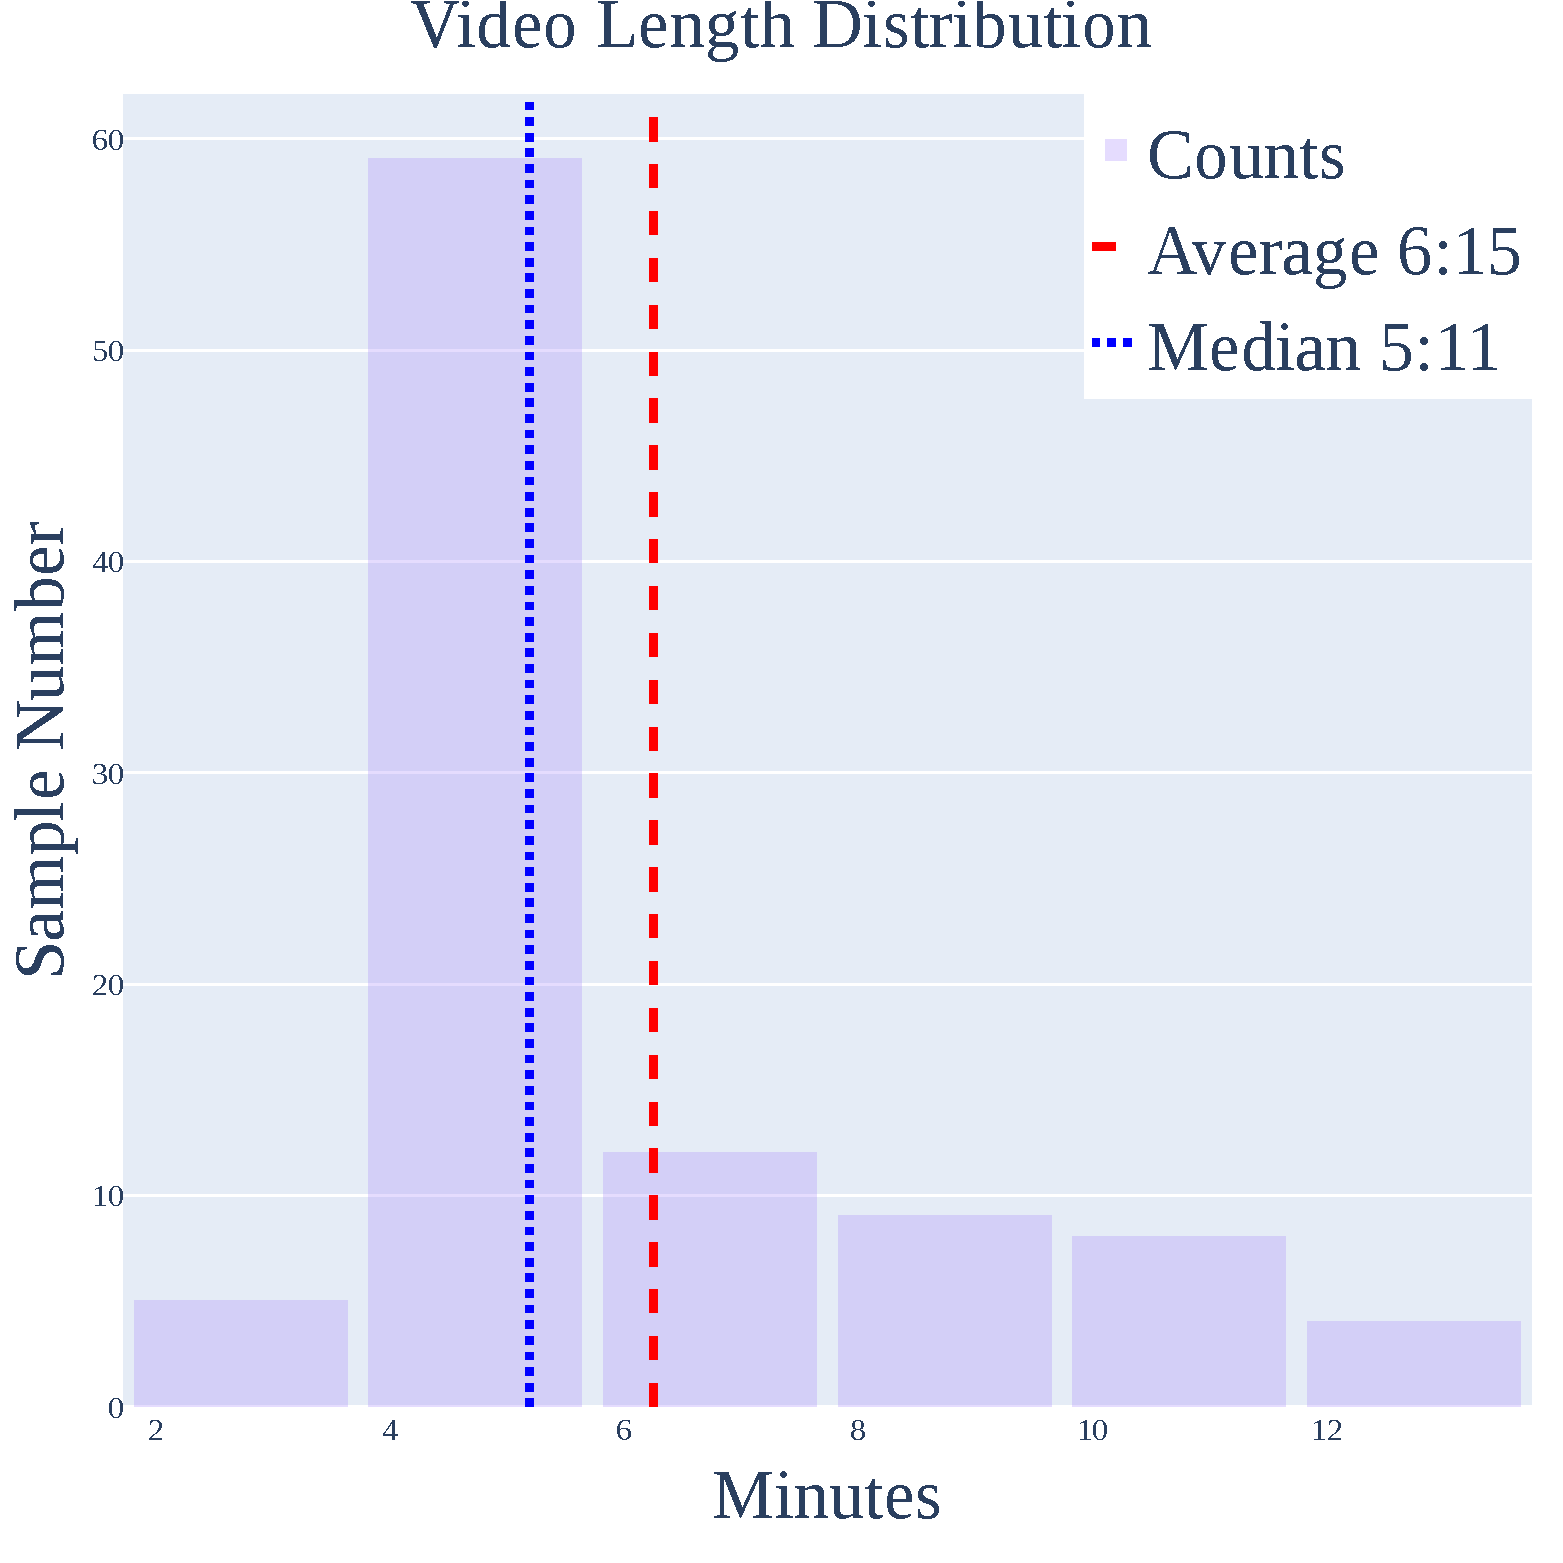
\includegraphics[width=0.30\textwidth]{figure/video_length_hist.pdf}
    \caption{Paper topics, slides per video, and video lengths in \alertterm{Paper2Video} benchmark.}
    \label{fig:stat}
  \end{figure}
  \vspace{-1\baselineskip}
   \scriptsize
  \begin{itemize}
    \item \alertterm{Paper2Video} (\bench): The first benchmark with \alertterm{101 research papers}, paired with author-created presentation videos, slides, and metadata.
    \item Curated from diverse AI conferences (\alertterm{ML, CV, NLP}), including videos, slides, portraits, and voice samples.
    \item Provides a platform to evaluate \alertterm{long-context, multimodal academic video generation} and new evaluation protocols.
  \end{itemize}
  
  \begin{itemize}
    \item Each paper averages 13.3K words, 44.7 figures, and 16 slides.
    \item Presentations last about 6 minutes on average.
  \end{itemize}
\end{frame}

\begin{frame}{{\bench} Metrics}
  \begin{itemize}
    \item \alertterm{Evaluation:}
      \begin{itemize}
          \item Meta Similarity (alignment to human-created content)
          \item PresentArena (pairwise quality contest via VideoLLM)
          \item PresentQuiz (information coverage via video QA)
          \item IP Memory (author/work recall)
      \end{itemize}
  \end{itemize}
  \vspace{0.2cm}
  \begin{figure}
    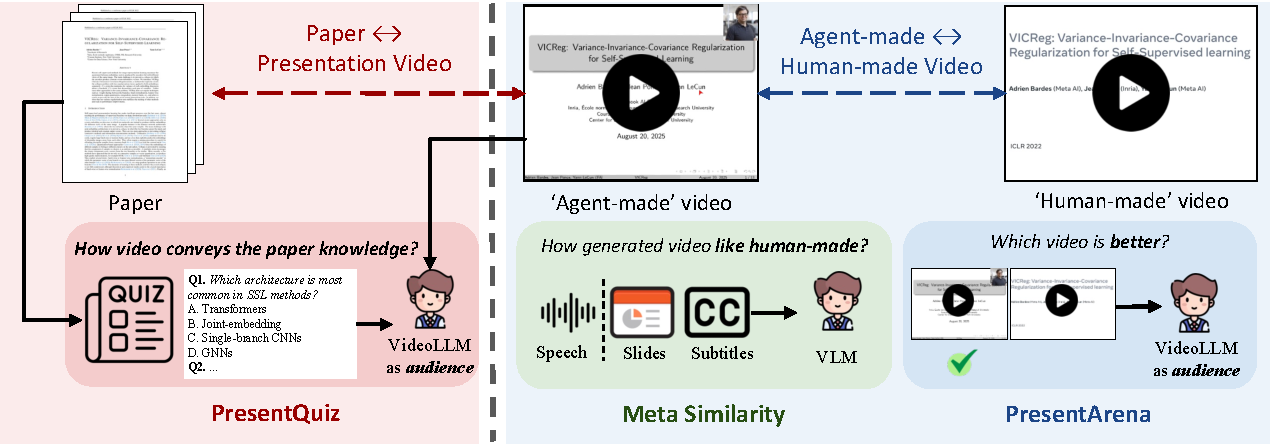
\includegraphics[width=0.65\textwidth]{figure/eval.pdf}
    \caption{Overview of \alertterm{evaluation metrics} in academic video generation.}
    \label{fig:eval}
  \end{figure}
\end{frame}

\begin{frame}{Method Overview: PaperTalker Agent}
  \begin{figure}
    \centering
    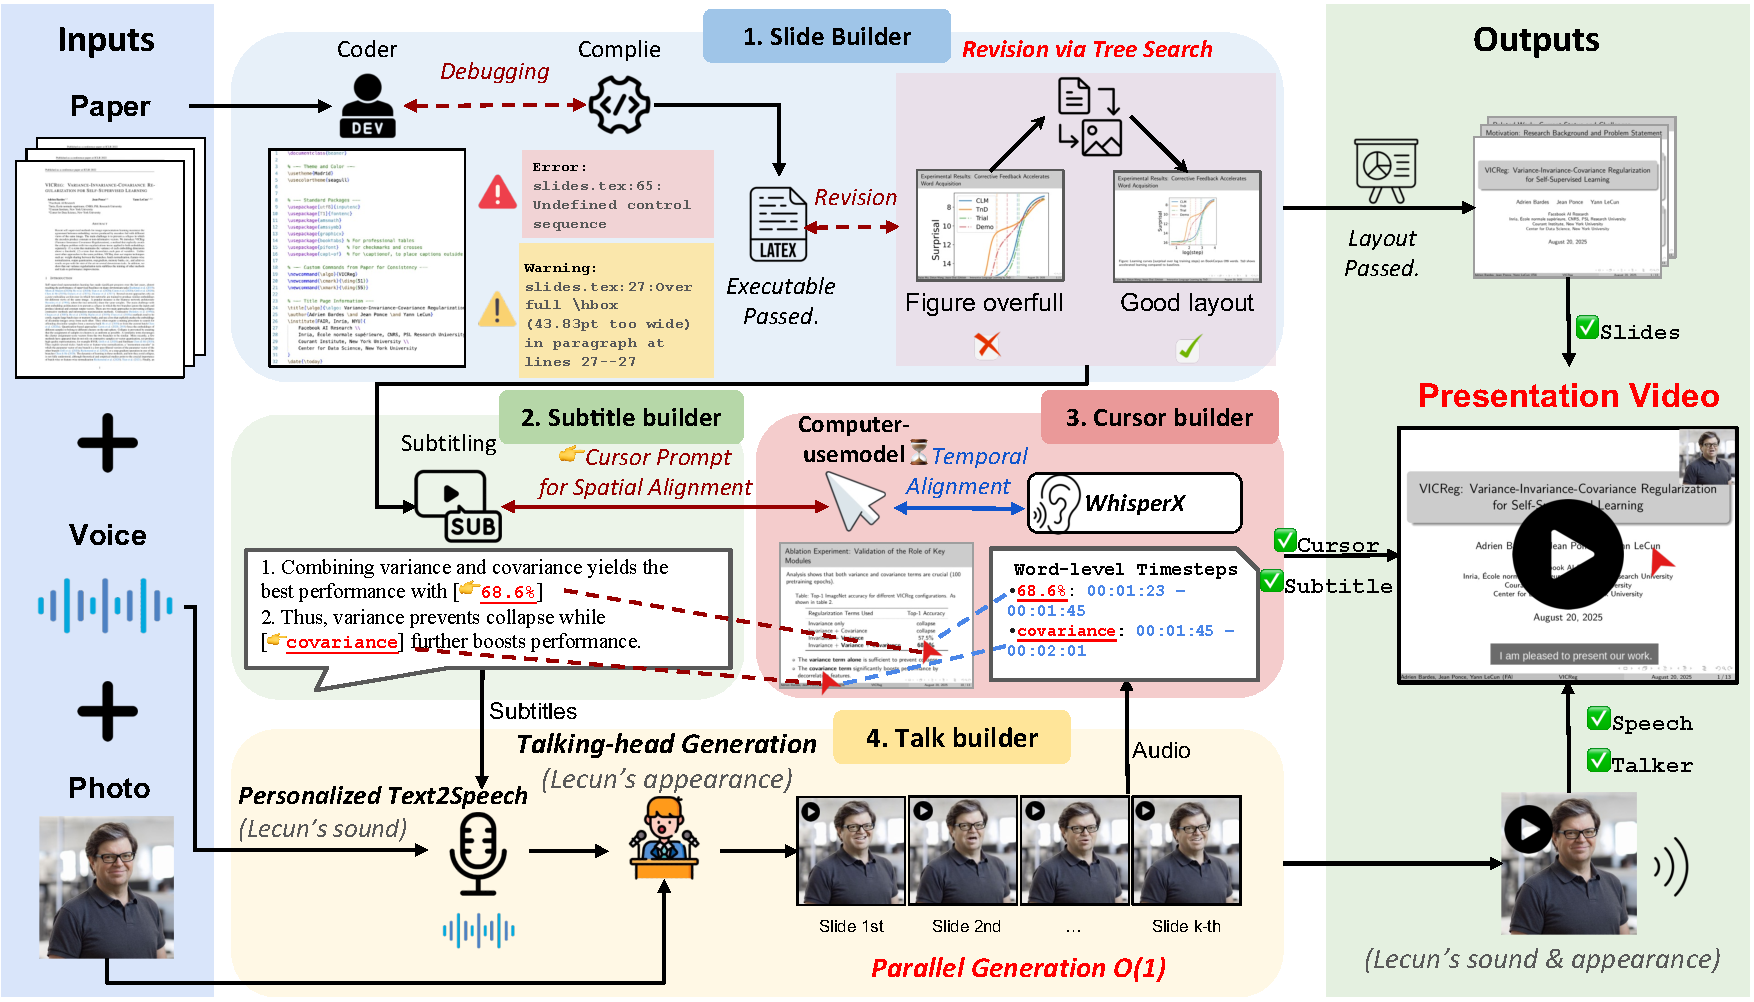
\includegraphics[width=0.7\textwidth]{figure/method.pdf}
    \caption{Overall pipeline of \alertterm{PaperTalker} for presentation video generation.}
    \label{fig:method}
  \end{figure}
  \vspace{-1 \baselineskip}
  \begin{block}{Key Modules}
    \scriptsize
    \begin{itemize}
      \item \alertterm{Slide Builder}: Generates slides in \LaTeX~Beamer, with visual layout refinement.
      \item \alertterm{Subtitle \& Cursor Builder}: Produces subtitles and aligns them with spatial-grounded cursor.
      \item \alertterm{Talker Builder}: Synthesizes speech and renders a personalized talking-head presenter.
      \item Supports \alertterm{slide-wise parallelization} for efficiency.
    \end{itemize}
  \end{block}
\end{frame}

\begin{frame}{Method: Slide Builder / Layout Refinement}
  \begin{itemize}
    \item \alertterm{Slides} created directly from paper's \LaTeX~source using Beamer for formal, academic layouts.
    \item Uses compiler feedback to iteratively fix issues.
    \item \alertterm{Tree Search Visual Choice}: A novel technique for fine-grained layout, exploring parameter variants and selecting the best with a vision-language model (VLM).
  \end{itemize}
  \begin{figure}
    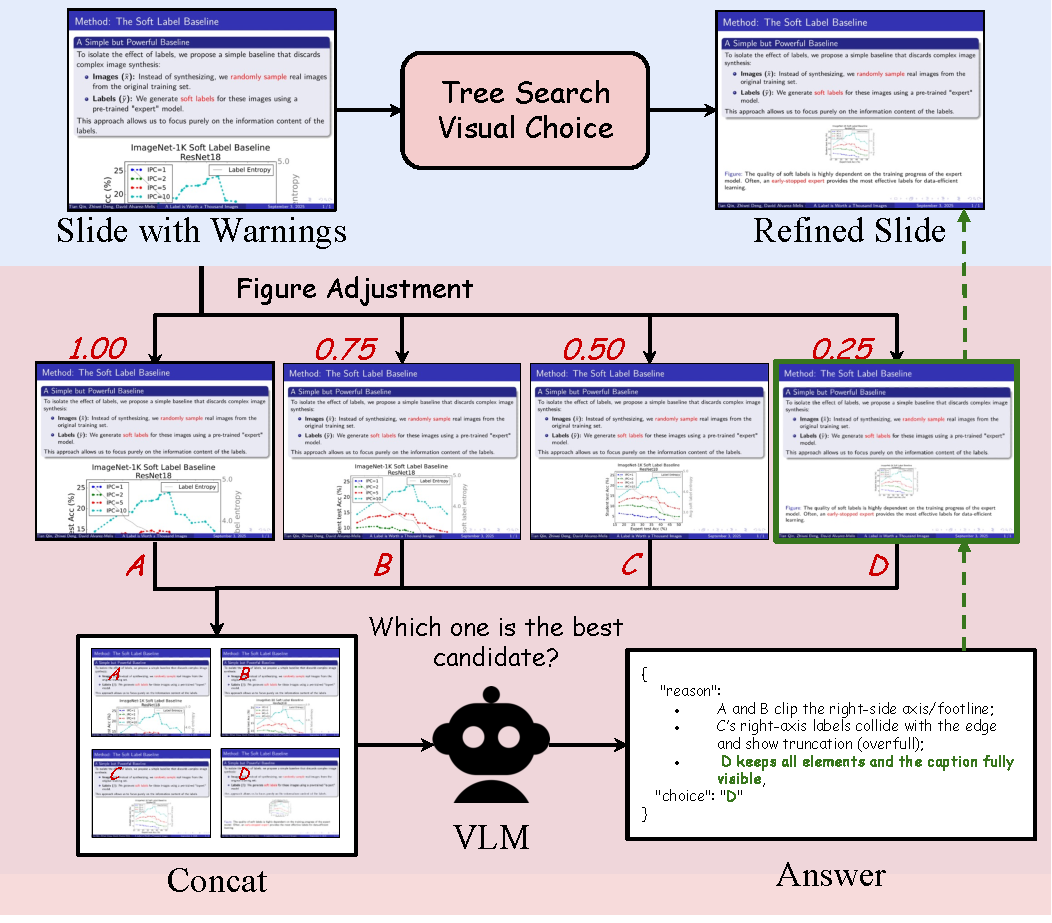
\includegraphics[width=0.5\textwidth]{figure/tree_search.pdf}
    \caption{\alertterm{Tree Search Visual Choice:} Visual refinement to resolve overfull/overflow slides.}
    \label{fig:mcts}
  \end{figure}
\end{frame}
\begin{frame}{Method: Subtitle and Cursor Builder}
  \begin{itemize}
    \item Subtitles are generated per slide, using a VLM to align content.
    \item \alertterm{Visual Focus Prompts} direct the cursor to key content.
    \item \alertterm{Cursor spatial-temporal alignment}: UI-TARS grounds cursor position, WhisperX aligns timing with narration.
  \end{itemize}
  \begin{block}{Benefit}
    \footnotesize
    \begin{itemize}
      \item \alertterm{Enhanced audience guidance} and accessibility.
    \end{itemize}
  \end{block}
\end{frame}
\begin{frame}{Method: Talker Builder \& Parallelization}
  \begin{itemize}
    \item Personalized speech synthesis using author voice sample (\alertterm{F5-TTS}), supporting slide granularity.
    \item Realistic talking-head generated with portrait (\alertterm{FantasyTalking, Hallo2}).
    \item \alertterm{Parallel per-slide synthesis} dramatically speeds up video generation.
  \end{itemize}
  \begin{figure}
    
\includegraphics[width=0.45\textwidth]{figure/presenter.png}
    \caption{Personalized \alertterm{talking-head} presenter output.}
    \label{fig:presenter}
  \end{figure}
\end{frame}
% \begin{frame}{Experimental Design}
%   \begin{itemize}
%     \item \alertterm{Baselines:}
%     \begin{itemize}
%       \item End-to-end video generation (e.g., Veo3)
%       \item Multi-agent methods (e.g., PresentAgent)
%       \item Human-created presentations for comparison
%     \end{itemize}
%     \item \alertterm{Evaluation:}
%       \begin{itemize}
%           \item Meta Similarity (alignment to human-created content)
%           \item PresentArena (pairwise quality contest via VideoLLM)
%           \item PresentQuiz (information coverage via video QA)
%           \item IP Memory (author/work recall)
%       \end{itemize}
%   \end{itemize}
%   \vspace{0.2cm}
%   \begin{figure}
%     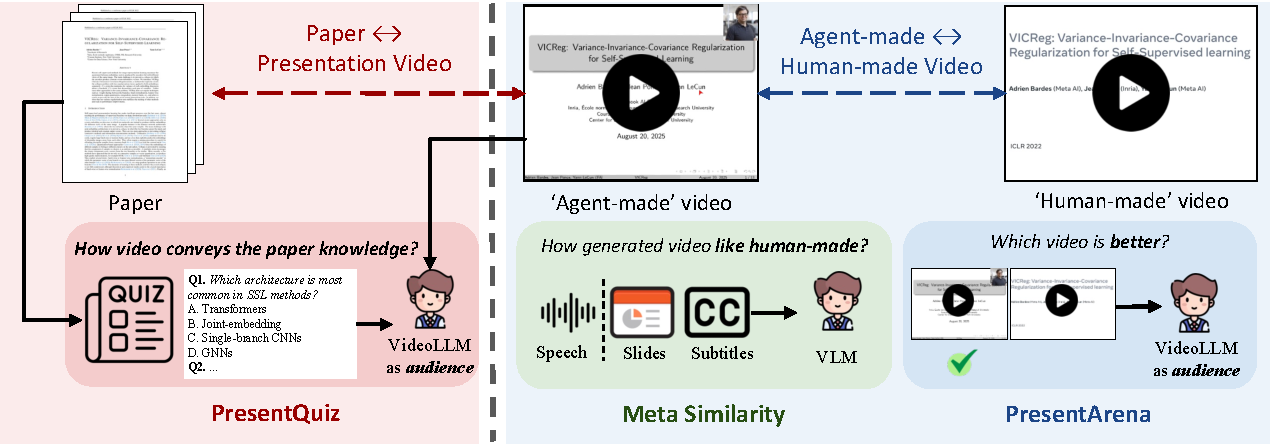
\includegraphics[width=0.5\textwidth]{figure/eval.pdf}
%     \caption{Overview of \alertterm{evaluation metrics} in academic video generation.}
%     \label{fig:eval}
%   \end{figure}
% \end{frame}
\begin{frame}{Experimental Settings}
  \begin{itemize}
    \item \alertterm{Baselines:}
    \begin{itemize}
      \item End-to-end video generation (e.g., Veo3)
      \item Multi-agent methods (e.g., PresentAgent)
      \item Human-created presentations for comparison
    \end{itemize}
    
    \item \alertterm{Dataset:} Paper2Video benchmark (\bench), 101 paper/video pairs.
    \item Hardware: 8$\times$ NVIDIA RTX A6000 GPUs.
    \item LLM/VLMs: All methods evaluated on same set; VideoLLM (Gemini-2.5-Flash), VLM (GPT-4.1).
  \end{itemize}
\end{frame}
\begin{frame}{Experimental Results: Main}
  \begin{table}[ht]
    \centering
    \tiny
    \label{tab:main_result}
    \caption{\textbf{Main Evaluation Results}. $\text{PaperTalk}^{*}$ represents a simple version without presenter and cursor.}
    \begin{tabular}{l c c c c c}
      \toprule
      Method & Sim. (Speech/Content) & Arena Win & PresentQuiz & IP Mem. & Dur. (s)\\
      \midrule
      HumanMade & \alertterm{1.00/5.00}  & \alertterm{50\%} & 0.738/0.908 & - & 375\\
      \midrule
      Wan2.2~\cite{wan} & NA/NA & 1.1\% & 0.251/0.551 & 11.5\% & 4.00\\
      Veo3      & 0.133/NA   & 1.2\%  & 0.367/0.585 & 31.3\% & 8\\
      PresentAgent & 0.045/1.47 & 2.0\%  & 0.548/0.654 & 12.5\% & 430\\
      PaperTalker* & \alertterm{0.646}/\alertterm{1.97} & 15.2\% & 0.835/0.949 & 37.5\% & 234\\
      PaperTalker & \alertterm{0.646}/\alertterm{1.97} & \alertterm{17.0\%} & \alertterm{0.842}/\alertterm{0.951} & \alertterm{50.0\%} & 234\\
      \bottomrule
    \end{tabular}
  \end{table}
  \vspace{0.1cm}
  % {\scriptsize
  %   \alertterm{PaperTalker} outperforms all baselines in both automatic and human evaluations.
  % }
  \begin{minipage}{0.5\linewidth}
    \centering
    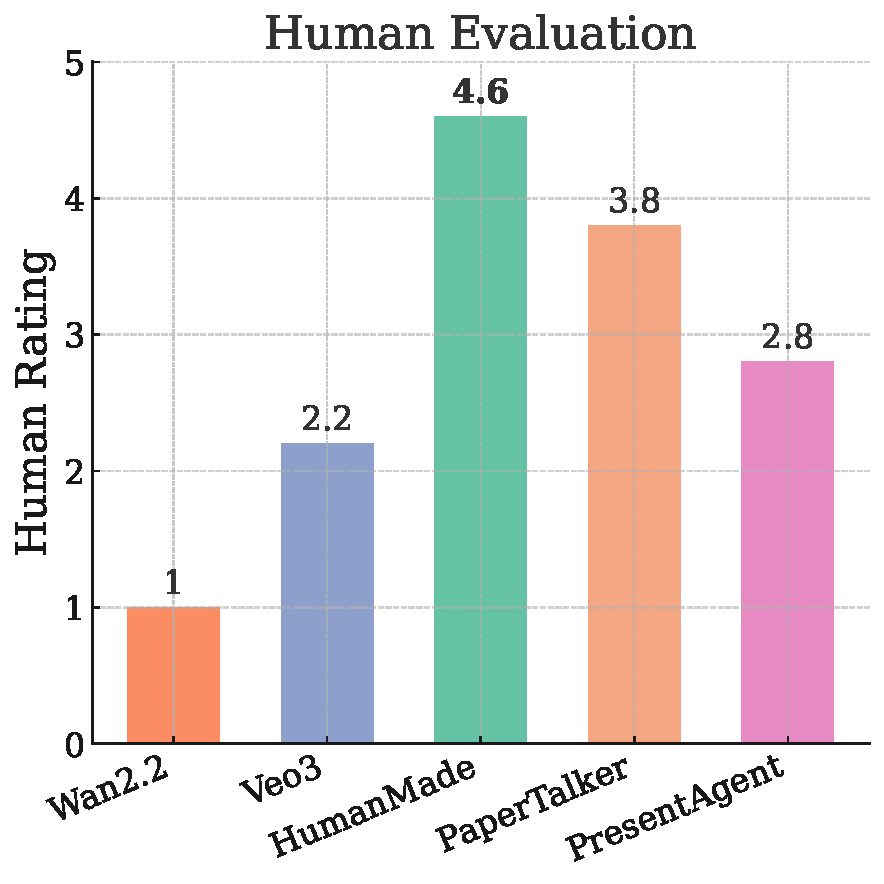
\includegraphics[width=0.7\linewidth]{figure/human_evaluation_bar.pdf}
  \end{minipage}%
  \hfill
  \begin{minipage}{0.45\linewidth}
    {\scriptsize
     \begin{itemize}
      \item \alertterm{PaperTalker} outperforms all baselines in both metric and human evaluations.
      \item Adding presenter video boosts engagement and quality preference by 10%.
      \end{itemize}
    }
  \end{minipage}
\end{frame}

\begin{frame}{Experimental Results: Efficiency}
  \begin{table}[h]
    \centering
    \small
    \setlength{\tabcolsep}{3pt}
    \caption{\textbf{Generation cost for each method.}}
    \begin{tabular}{lccc}
      \toprule
      Method & Token (K)$\downarrow$ & Time (min.)$\downarrow$ & Cost (\$)$\downarrow$ \\
      \midrule
      Veo3~\cite{deepmind2025veo3} & NA & \textbf{0.4} & 1.667 \\
      Wan2.2~\cite{wan} & NA & 8.1 & 0.280 \\
      \midrule
      PresentAgent~\cite{shi2025presentagent} & 241 & 39.5 & 0.003  \\
      PaperTalker (w/o Talker) & \textbf{62} & 15.6 & \textbf{0.001}\\    
      \midrule
      PaperTalker (w/o Par.) & \textbf{62} & 287.2 & \textbf{0.001}\\
      PaperTalker & \textbf{62} & 48.1 \textbf{(\alertterm{6$\times$})} & \textbf{0.001} \\
      \bottomrule
    \end{tabular}
    \label{table:cost}
  \end{table}

  \vspace{-0.3\baselineskip}
  \small
  \textbf{Efficiency Highlights:}
  \begin{itemize}
    \item \textbf{Speed vs. PresentAgent:} 39.5 $\rightarrow$ 15.6 min (2.5$\times$ faster).  
    \item \textbf{Parallel Generation:} 287.2 $\rightarrow$ 48.1 min (\textbf{6$\times$ speedup}).  
    \item \textbf{Lowest Cost:} Only \$0.001, cheapest among all methods.  
  \end{itemize}
\end{frame}




\begin{frame}{Ablation Study: Cursor and Tree Search}
  \begin{columns}[T] % T=top aligned
    % 左边 bullet
    \begin{column}{0.4\textwidth}
      \small
      \begin{itemize}
        \item \textbf{Cursor Highlight}: Markedly improves content localization (QA acc. rises from 8\% to 63\%).\\
        \item \textbf{Slide Quality}: Tree search refinement fixes layout issues and improves coherence.
      \end{itemize}
    \end{column}

    % 右边两个表格堆叠
    \begin{column}{0.6\textwidth}
      \centering
      \scriptsize
      % 小表格:Cursor
      % \captionof{table}{\textbf{Ablation study on cursor.}}
      % \vspace{-0.5\baselineskip}
      \tiny
      \setlength{\tabcolsep}{2pt}
      {\scriptsize \textbf{Table:} Ablation study on cursor.}
      \begin{tabular}{lc}
        \toprule
        Method & Accuracy$\uparrow$ \\
        \midrule
        PaperTalker (w/o Cursor) & 0.084 \\
        PaperTalker & \textbf{0.633} \\
        \bottomrule
      \end{tabular}

      \vspace{0.8\baselineskip}

      % 大表格:Slide Quality
    \begin{table}
      \centering
      \tiny
      \setlength{\tabcolsep}{2pt}
      {\scriptsize \textbf{Table:} Evaluation result on slide quality.}
      \vspace{2pt} % 表格和 caption 的间距
      \begin{tabular}{lccc}
        \toprule
        Method & Content ($\uparrow$) & Design ($\uparrow$) & Coherence ($\uparrow$) \\
        \midrule
        HumanMade & \textbf{4.43} & \textbf{2.85} & 2.73 \\
        \midrule
        $\text{PPTAgent}_\text{Qwen7B}$ & 3.43 & 1.57 & 1.29 \\
        $\text{PaperTalker}_\text{Qwen7B}$ & 4.00 & 2.53 & \underline{3.11} \\
        \midrule
        $\text{PPTAgent}_\text{GPT4.1}$ & 4.07 & 2.02 & 2.06 \\
        $\text{PaperTalker}_\text{GPT4.1}$(w/o TS) & 4.33 & \underline{2.73} & \textbf{3.84} \\
        $\text{PaperTalker}_\text{GPT4.1}$ & \underline{4.34} & \textbf{2.85} & \textbf{3.84} \\
        \bottomrule
      \end{tabular}

    \end{table}
    \end{column}
  \end{columns}
\end{frame}

\begin{frame}{Visualization Comparison: Main Result}
  \begin{figure}
    \centering
    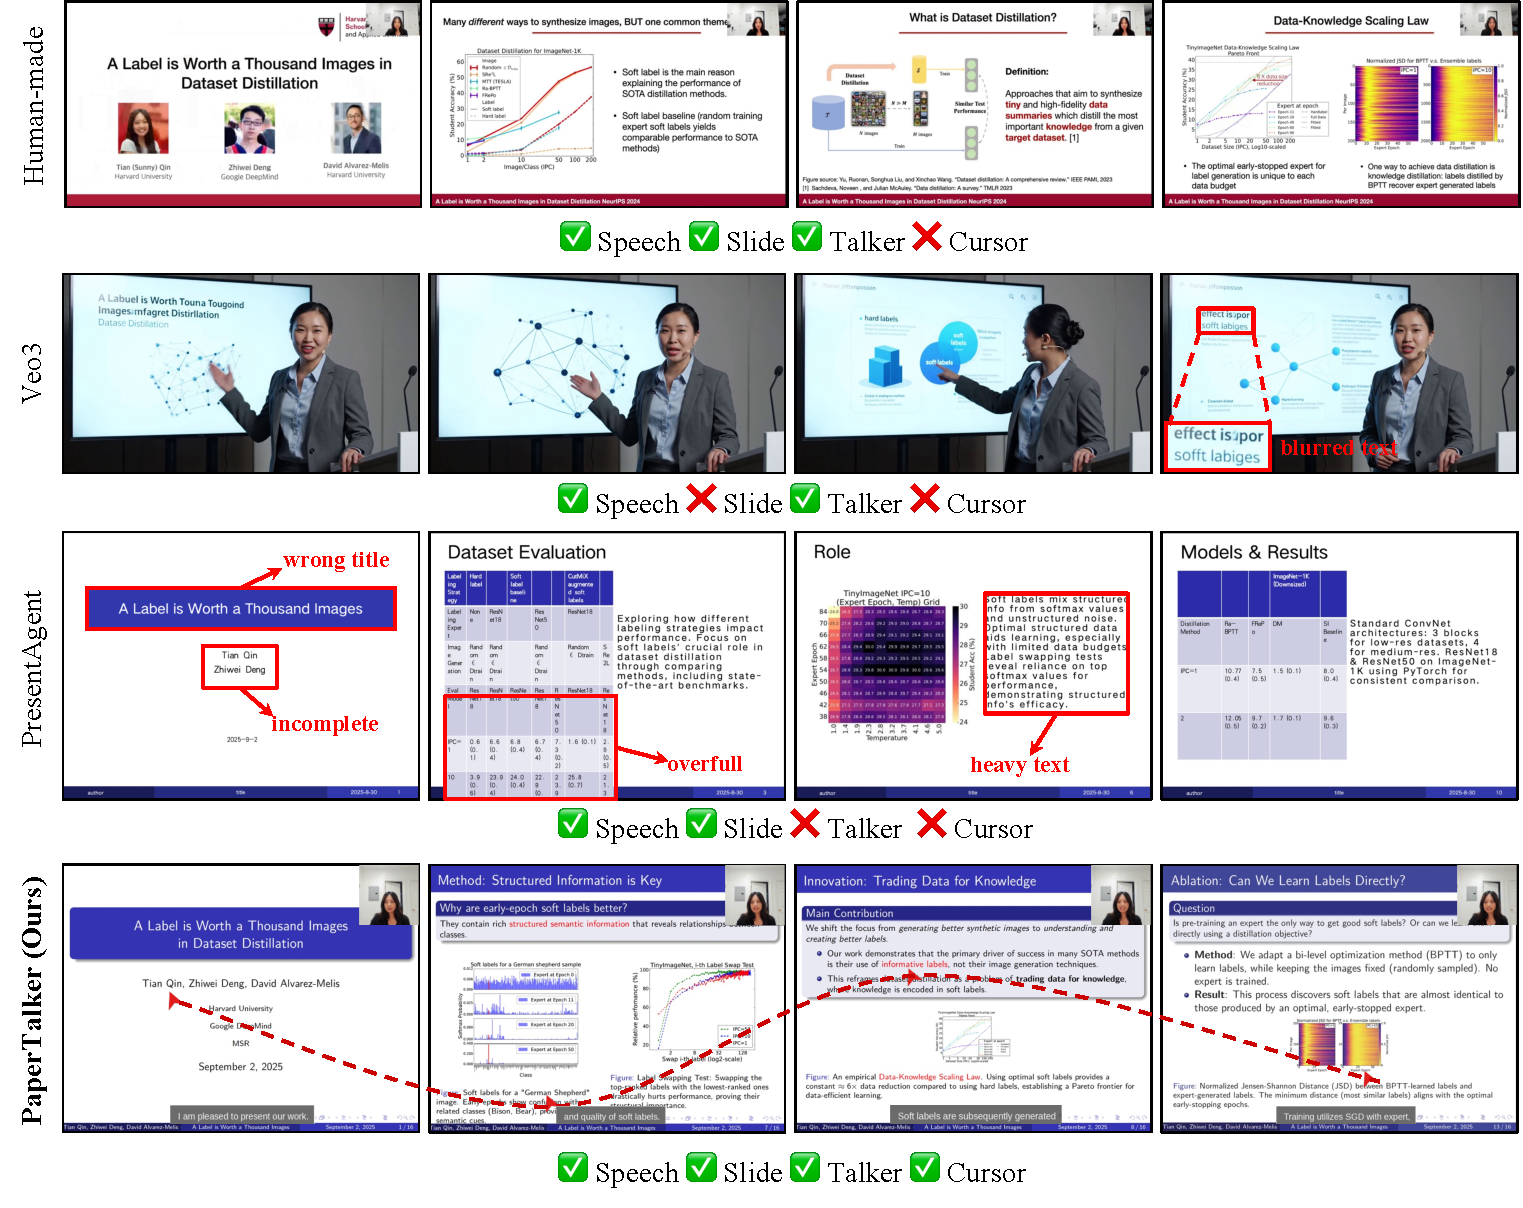
\includegraphics[width=0.7\linewidth]{figure/vis.pdf}
    \caption{\textbf{Visualization of generated results.} PaperTalker produces slides with rich content, accurate cursor grounding, and an engaging talker. In contrast, Veo3 shows blurred text and incomplete coverage, while PresentAgent yields text-heavy slides with layout issues and inaccurate information (\textit{e.g.}, title and institution).}
  \end{figure}
\end{frame}


\begin{frame}{Visualization Comparison: Tree Search}
 \begin{figure}
     \centering
     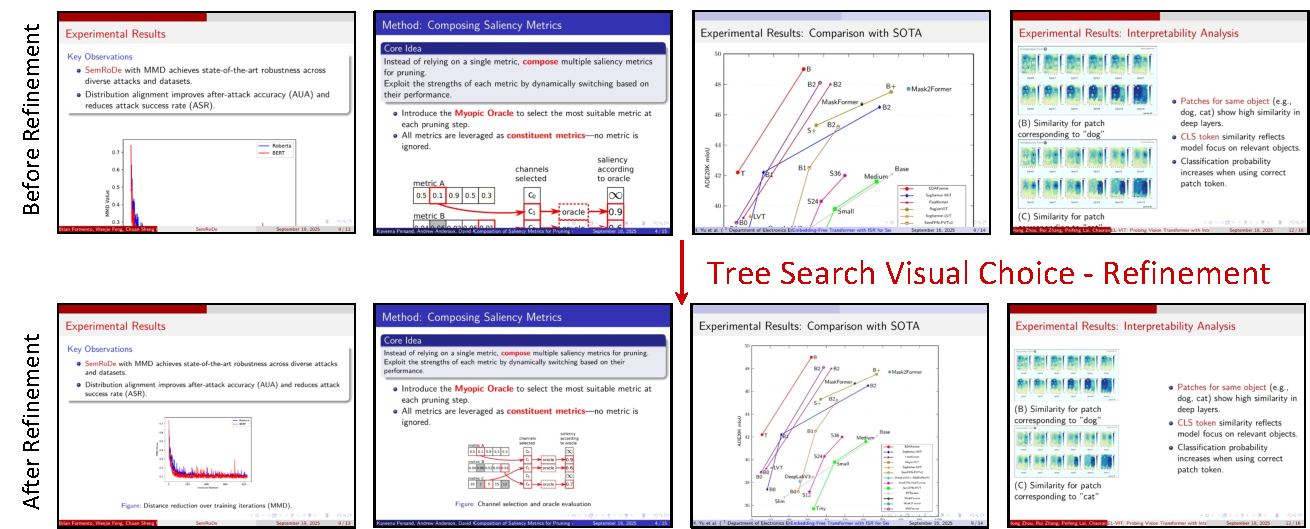
\includegraphics[width=1\linewidth]{figure/tree_search_vis.pdf}
     \caption{\textbf{Slide Visualization of Tree Search Visual Choice.} The first row shows slide results before layout refinement, while the second row shows their corresponding slides after refinement.}
     \label{fig:placeholder}
 \end{figure}
\end{frame}

\begin{frame}{Limitations and Future Work}
  \begin{itemize}
    \item \alertterm{Limitations}. Long-document parsing and highly technical equations remain challenging for end-to-end generation.
     \item \alertterm{Future Work}. Real-time interactive video agents for tutorial or Q\&A sessions.
  \end{itemize}
\end{frame}
% \begin{frame}{Future Work}
%   \begin{itemize}
%     \item Enhanced \alertterm{semantic understanding} for even longer, more complex papers.
%     \item Improved \alertterm{multilingual support} and accessibility features.
%     \item Real-time interactive video agents for tutorial or Q\&A sessions.
%     \item Closed-loop evaluation protocols involving both humans and intelligent audience proxies.
%     \item Full open-sourcing to empower the research community and collaborative development.
%   \end{itemize}
% \end{frame}
\begin{frame}
  \centering
  \Huge \textbf{Thank You!}
  \vspace{0.7cm}

  
\includegraphics[width=0.15\textwidth]{figure/logo_.png}

  \vspace{0.3cm}
  \large
  \texttt{Questions and Discussion Welcome.} \\
  \href{mailto:showlab@nus.edu.sg}{e1374425@nus.edu.sg}
\end{frame}
\end{document}